% \subsubsection{Core Components}
Kubernetes is complex and resource intensive tool. However, much of the resource overhead stems from the control plane which only runs on master nodes. These nodes are not in the scope of this thesis and thus not explained in more detail. Worker nodes on the other hand are orchestrated and provide their state to the master. This is a lot less resource intensive and there are a few tricks to reduce the resource load even further. For a worker node to be part of a cluster it needs to run the following components: the \textit{kubelet}, \textit{kube-proxy} and a supported container runtime. How Kubernetes works in practice can be seen in \cref{fig:nodeComponents}\footnote{The \textit{cAdvisor} component is a health checking tool and not required.}.
\begin{figure}[h!]
    \centering
    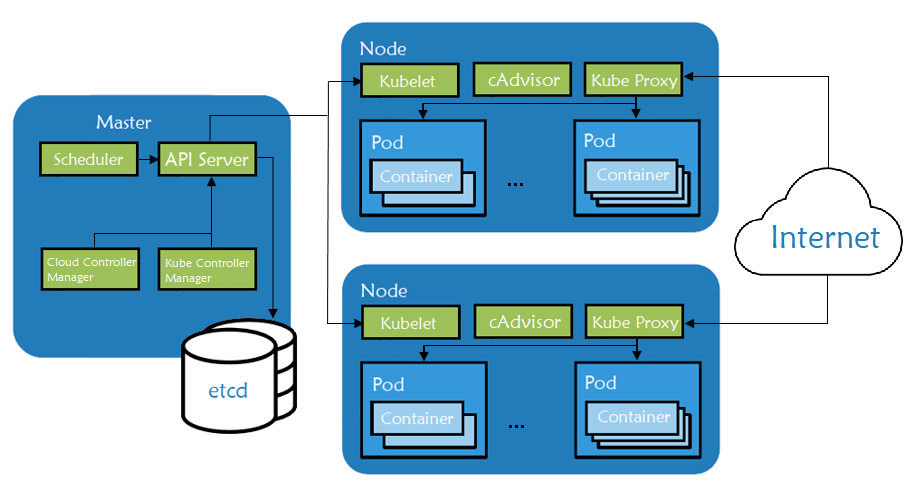
\includegraphics[scale=0.6]{figures/rancherK8sComponents.png}
    \caption{The Kubernetes architecture and node components\cite{nodeSetupKubernetes:online}}
    \label{fig:nodeComponents}
\end{figure}
The kubelet is the primary node agent and schedules and maintains containers running inside a pod based on the pods \textit{PodSpecs}. It gets the these specifications mainly from the APIServer, but other Kubernetes internal sources are possible, too. Containers created outside of the cluster (or multi cluster) are not managed by the kubelet. 

Configuring the kubelet is easily possible via the kubectl and kubeadm tools which give the possibility of enhancing the kubelets performance for different circumstances, e.g. the edge. Going through the possible configurations under \url{https://kubernetes.io/docs/reference/command-line-tools-reference/kubelet/}, the most important configurations for the edge is the \textit{--housekeeping-interval duration} which defaults to 10s\cite{rancherKubernetesComponents:online}. This means each 10 seconds the kubelet performs a complete health check of all its components and sends it to the master. For normal cloud nodes this is a sensible choice. The nodes are powerful enough to handle the additional overhead and it avoids having unavailable resources. For light edge devices the interval is too high. The kubelet from k3s (discussed in \cref{sec:existingSolutions}) called hypervisor is compatible with vanilla Kubernetes and optimized for light edge devices.

For networking Kubernetes provides the kube-proxy which is a network proxy node agent ensuring that the Kubernetes networking services run on each node. It enables the Kubernetes service abstraction by ensuring the network rules on each host and carries out the connection forwarding. Kubernetes does not provide a standard implementation but requires the administrator to provide one at the installation. The last component, the container runtime (discussed in the \cref{sec:containers}), ensures that containers can run as expected.



